\begin{tomtat}
	\begin{minipage}[t]{0.3\textwidth}
		\vspace{0pt}
		\begin{tomtat}
			\begin{center}
				\textbf{ĐỀ 19}
			\end{center}
			
		\end{tomtat}
	\end{minipage}
	\hfill
	\begin{minipage}[t]{0.5\textwidth}
		\vspace{0pt}
		\begin{tomtat}
			\begin{center}
				\includegraphics[scale=0.08]{images/19}
			\end{center}
		\end{tomtat}
	\end{minipage}
\end{tomtat}
\textbf{I. PHẦN TRẮC NGHIỆM}
\begin{ex} % Câu 1
	Kết quả rút gọn biểu thức $A=\sqrt{45}-2\sqrt{5}$ là:
	\choice{$-\sqrt{5}$}{$\sqrt{5}$}{$2\sqrt{5}$}{$-2\sqrt{5}$}
	\loigiai{
		Ta có:
		\begin{align*}
			A &= \sqrt{45}-2\sqrt{5} \\
			&= \sqrt{9 \cdot 5} - 2\sqrt{5} \\
			&= 3\sqrt{5} - 2\sqrt{5} \\
			&= (3-2)\sqrt{5} \\
			&= \sqrt{5}
		\end{align*}
		\\ \textbf{ĐÁP ÁN B}
	}
\end{ex}

\begin{ex} % Câu 2
	Nghiệm của phương trình: $2x - 1 = 3$ là:
	\choice{1}{-1}{2}{-2}
	\loigiai{
		Ta giải phương trình:
		\begin{align*}
			2x - 1 &= 3 \\
			2x &= 3+1 \\
			2x &= 4 \\
			x &= \frac{4}{2} \\
			x &= 2
		\end{align*}
		Vậy nghiệm của phương trình là $x=2$.
		\\ \textbf{ĐÁP ÁN C}
	}
\end{ex}

\begin{ex} % Câu 3
	Đồ thị hàm số $y=-2x^2$ đi qua điểm nào sau đây:
	\choice{(1;2)}{(-1;2)}{(1;-2)}{(1;-2)} 
	% Lưu ý: Đáp án C và D giống nhau trong ảnh.
	\loigiai{
		Ta thay tọa độ các điểm vào phương trình hàm số $y=-2x^2$:
		\begin{itemize}
			\item A. Điểm (1;2): $2 = -2(1)^2 \Rightarrow 2 = -2$ (Sai).
			\item B. Điểm (-1;2): $2 = -2(-1)^2 \Rightarrow 2 = -2(1) \Rightarrow 2 = -2$ (Sai).
			\item C. Điểm (1;-2): $-2 = -2(1)^2 \Rightarrow -2 = -2(1) \Rightarrow -2 = -2$ (Đúng).
			\item D. Điểm (1;-2): $-2 = -2(1)^2 \Rightarrow -2 = -2(1) \Rightarrow -2 = -2$ (Đúng).
		\end{itemize}
		Vậy đồ thị hàm số đi qua điểm (1;-2).
		\\ \textbf{ĐÁP ÁN D} (Hoặc C)
	}
\end{ex}

\begin{ex} % Câu 4
	Một đĩa tròn bằng bìa cứng được chia làm 12 phần bằng nhau và ghi các số 1, 2, 3, ..., 12; chiếc kim được gắn cố định vào trục quay ở tâm của đĩa. Xét phép thử “Quay đĩa tròn một lần”. Gọi biến cố A “Chiếc kim chỉ vào hình quạt ghi số chia hết cho 3”. Số kết quả thuận lợi cho biến cố A là:
	\choice{2}{3}{4}{5}
	\loigiai{
		Các số ghi trên đĩa là $\{1, 2, 3, 4, 5, 6, 7, 8, 9, 10, 11, 12\}$.
		Biến cố A: “Chiếc kim chỉ vào hình quạt ghi số chia hết cho 3”.
		Các số chia hết cho 3 trong tập hợp trên là: $\{3, 6, 9, 12\}$.
		Số kết quả thuận lợi cho biến cố A là 4.
		\\ \textbf{ĐÁP ÁN C}
	}
\end{ex}

\begin{ex} % Câu 5
	Cho tam giác ABC vuông tại A. Biết AC=8cm, BC=12cm, $\cos C$ bằng:
	\choice{$\frac{3}{2}$}{$\frac{2}{3}$}{$\frac{3}{4}$}{$\frac{4}{3}$}
	\loigiai{
		Trong tam giác ABC vuông tại A:
		Theo định nghĩa tỉ số lượng giác cosin, ta có:
		$$ \cos C = \frac{\text{cạnh kề}}{\text{cạnh huyền}} = \frac{AC}{BC} $$
		Với $AC=8 \text{ cm}$ và $BC=12 \text{ cm}$, ta có:
		$$ \cos C = \frac{8}{12} = \frac{2}{3} $$
		\\ \textbf{ĐÁP ÁN B}
	}
\end{ex}

\begin{ex} % Câu 6
	Tính thể tích hình trụ có bán kính đáy 4cm, chiều cao 10cm là:
	\choice{$120\pi \text{ cm}^3$}{$160\pi \text{ cm}^3$}{$140\pi \text{ cm}^3$}{$144\pi \text{ cm}^3$}
	\loigiai{
		Thể tích của hình trụ được tính bằng công thức: $V = \pi R^2 h$.
		Trong đó $R$ là bán kính đáy ($R=4 \text{ cm}$) và $h$ là chiều cao ($h=10 \text{ cm}$).
		\begin{align*}
			V &= \pi (4)^2 \cdot 10 \\
			&= \pi \cdot 16 \cdot 10 \\
			&= 160\pi (\text{cm}^3)
		\end{align*}
		\\ \textbf{ĐÁP ÁN B}
	}
\end{ex}

\begin{ex} % Câu 7
	Nghiệm của bất phương trình $-3x+6>0$ là:
	\choice{$x>2$}{$x<2$}{$x \ge 2$}{$x \le 2$}
	\loigiai{
		Ta giải bất phương trình:
		\begin{align*}
			-3x+6 &> 0 \\
			-3x &> -6
		\end{align*}
		Khi chia cả hai vế của bất phương trình cho một số âm (ở đây là -3), ta phải đổi chiều bất đẳng thức:
		\begin{align*}
			x &< \frac{-6}{-3} \\
			x &< 2
		\end{align*}
		Vậy nghiệm của bất phương trình là $x<2$.
		\\ \textbf{ĐÁP ÁN B}
	}
\end{ex}
\begin{ex}
	Thống kê điểm kiểm tra định kỳ môn Toán của học sinh lớp 9B như sau:
	\begin{center}
		\begin{tabular}{|c|c|c|c|c|c|c|c|c|c|}
			\hline
			5 & 5 & 5 & 7 & 7 & 8 & 8 & 8 & 5 & 8 \\
			\hline
			8 & 8 & 6 & 6 & 6 & 6 & 8 & 9 & 5 & 7 \\
			\hline
			6 & 6 & 7 & 7 & 6 & 8 & 9 & 9 & 7 & 8 \\
			\hline
			8 & 5 & 7 & 7 & 7 & 7 & 6 & 8 & 8 & 9 \\
			\hline
		\end{tabular}
	\end{center}
	Tần số của giá trị 9 điểm là:
	\choice{2}{3}{4}{5}
	
	\loigiai{
		Đếm số lần xuất hiện của điểm 9 trong bảng thống kê:
		\begin{itemize}
			\item Hàng thứ nhất: 0 lần xuất hiện điểm 9.
			\item Hàng thứ hai: 1 lần xuất hiện điểm 9.
			\item Hàng thứ ba: 2 lần xuất hiện điểm 9.
			\item Hàng thứ tư: 1 lần xuất hiện điểm 9.
		\end{itemize}
		Tổng số lần xuất hiện điểm 9 là: $0 + 1 + 2 + 1 = 4$ lần.
		Vậy, tần số của giá trị 9 điểm là 4.
		\\ \textbf{Đáp Án C}
	}
\end{ex}
\newpage
\textbf{II. PHẦN TỰ LUẬN}
\begin{ex} Rút gọn biểu thức:
	$$ P = \left( \frac{1}{x - \sqrt{x}} + \frac{1}{\sqrt{x} - 1} \right) : \frac{\sqrt{x}}{x - 2\sqrt{x} + 1} \quad (\text{với } x > 0, x \neq 1) $$
	\loigiai{
		Điều kiện: $x > 0, x \neq 1$.
		Ta có:
		\begin{align*} P &= \left( \frac{1}{\sqrt{x}(\sqrt{x} - 1)} + \frac{\sqrt{x}}{\sqrt{x}(\sqrt{x} - 1)} \right) : \frac{\sqrt{x}}{(\sqrt{x} - 1)^2} \\ &= \left( \frac{1 + \sqrt{x}}{\sqrt{x}(\sqrt{x} - 1)} \right) \cdot \frac{(\sqrt{x} - 1)^2}{\sqrt{x}} \\ &= \frac{(1 + \sqrt{x})\cancel{(\sqrt{x} - 1)}}{\sqrt{x}\cancel{(\sqrt{x} - 1)}} \cdot \frac{(\sqrt{x} - 1)}{\sqrt{x}} \\ &= \frac{1 + \sqrt{x}}{\sqrt{x}} \cdot \frac{\sqrt{x} - 1}{\sqrt{x}} \\ &= \frac{(1 + \sqrt{x})(\sqrt{x} - 1)}{\sqrt{x} \cdot \sqrt{x}} \\ &= \frac{(\sqrt{x})^2 - 1^2}{x} \\ &= \frac{x - 1}{x}\end{align*}
		Vậy $P = \frac{x-1}{x}$.
	}
\end{ex}
\begin{ex} Giải hệ phương trình:
	$$ \begin{cases} 3x + y = 5 \\ x - 2y = -3 \end{cases} $$
	\loigiai{
		Ta có hệ phương trình:
		$$ \begin{cases} 3x + y = 5 \quad &(1) \\ x - 2y = -3 \quad &(2) \end{cases} $$
		Từ phương trình (1), ta có $y = 5 - 3x$.
		Thế $y = 5 - 3x$ vào phương trình (2), ta được:
		$x - 2(5 - 3x) = -3$
		$x - 10 + 6x = -3$
		$7x = -3 + 10$
		$7x = 7$
		$x = 1$
		Thay $x = 1$ vào $y = 5 - 3x$, ta được:
		$y = 5 - 3(1) = 5 - 3 = 2$.
		Vậy nghiệm của hệ phương trình là $(x, y) = (1, 2)$.
	}
\end{ex}

\begin{ex} Giả sử phương trình $-3x^2 + x + 1 = 0$ có hai nghiệm là $x_1$ và $x_2$. Không giải phương trình, hãy tính giá trị biểu thức $A = x_1^2 - \frac{2}{x_1} + x_2^2 - \frac{2}{x_2}$.
	\loigiai{
		Phương trình đã cho là $-3x^2 + x + 1 = 0$.
		Vì $a \cdot c = (-3) \cdot 1 = -3 < 0$ nên phương trình luôn có hai nghiệm phân biệt $x_1, x_2$ (khác 0 vì $c=1 \neq 0$).
		Theo hệ thức Vi-ét, ta có:
		$$ \begin{cases} x_1 + x_2 = -\frac{b}{a} = -\frac{1}{-3} = \frac{1}{3} \\ x_1 x_2 = \frac{c}{a} = \frac{1}{-3} = -\frac{1}{3} \end{cases} $$
		Xét biểu thức A:
		\begin{align*} A &= x_1^2 - \frac{2}{x_1} + x_2^2 - \frac{2}{x_2} \\ &= (x_1^2 + x_2^2) - 2\left(\frac{1}{x_1} + \frac{1}{x_2}\right) \\ &= \left((x_1 + x_2)^2 - 2x_1x_2\right) - 2\left(\frac{x_1 + x_2}{x_1x_2}\right)\end{align*}
		Thay giá trị từ hệ thức Vi-ét vào biểu thức A:
		\begin{align*} A &= \left(\left(\frac{1}{3}\right)^2 - 2\left(-\frac{1}{3}\right)\right) - 2\left(\frac{\frac{1}{3}}{-\frac{1}{3}}\right) \\ &= \left(\frac{1}{9} + \frac{2}{3}\right) - 2(-1) \\ &= \left(\frac{1}{9} + \frac{6}{9}\right) + 2 \\ &= \frac{7}{9} + 2 \\ &= \frac{7}{9} + \frac{18}{9} \\ &= \frac{25}{9}\end{align*}
		Vậy $A = \frac{25}{9}$.
	}
\end{ex}
\begin{ex} Một xe lửa cần vận chuyển một lượng hàng. Người lái xe tính rằng nếu xếp mỗi toa 15 tấn thì còn thừa lại 5 tấn. Nếu xếp mỗi toa 16 tấn thì có thể chở thêm 3 tấn. Hỏi xe lửa có mấy toa và phải chở bao nhiêu tấn hàng?
	\loigiai{
		Gọi số toa xe lửa là $x$ (toa) (điều kiện $x \in \mathbb{N}^*$).
		Gọi tổng số tấn hàng cần chở là $y$ (tấn) (điều kiện $y > 0$).
		
		Theo đề bài, nếu xếp mỗi toa 15 tấn thì còn thừa lại 5 tấn, ta có phương trình:
		$y = 15x + 5 \quad (1)$
		
		Nếu xếp mỗi toa 16 tấn thì có thể chở thêm 3 tấn, nghĩa là tổng lượng hàng chở được ($16x$ tấn) nhiều hơn lượng hàng thực tế cần chở ($y$ tấn) là 3 tấn. Ta có phương trình:
		$16x = y + 3 \implies y = 16x - 3 \quad (2)$
		
		Từ (1) và (2), ta có hệ phương trình:
		$$ \begin{cases} y = 15x + 5 \\ y = 16x - 3 \end{cases} $$
		Trừ vế theo vế của hai phương trình, hoặc thế $y$ từ phương trình (1) vào phương trình (2), ta được:
		$15x + 5 = 16x - 3$
		$16x - 15x = 5 + 3$
		$x = 8$
		
		Thay $x = 8$ vào phương trình (1):
		$y = 15(8) + 5 = 120 + 5 = 125$.
		
		Kiểm tra lại với $x=8, y=125$:
		Phương trình (1): $125 = 15(8) + 5 \Leftrightarrow 125 = 120 + 5 \Leftrightarrow 125 = 125$ (Đúng).
		Phương trình (2): $125 = 16(8) - 3 \Leftrightarrow 125 = 128 - 3 \Leftrightarrow 125 = 125$ (Đúng).
		
		Vậy xe lửa có 8 toa và phải chở 125 tấn hàng.
	}
\end{ex}
\begin{ex} Một hộp có 20 viên bi với kích thước và khối lượng như nhau. Bạn Ngân viết lên các viên bi đó các số 1, 2, 3, ..., 20; hai viên bi khác nhau thì viết hai số khác nhau. Xét phép thử “Lấy ngẫu nhiên một viên bi trong hộp”. Tính xác suất biến cố: “Số xuất hiện trên viên bi được lấy ra chia 7 dư 1”.
	\loigiai{
		Không gian mẫu $\Omega = \{1; 2; 3; 4; 5; 6; 7; 8; 9; 10; 11; 12; 13; 14; 15; 16; 17; 18; 19; 20\}$. \\
		Số phần tử của không gian mẫu là  $n(\Omega) = 20$. \\
		Gọi A là biến cố: “Số xuất hiện trên viên bi được lấy ra chia 7 dư 1”.\\
		Do đó, các kết quả thuận lợi cho biến cố A là $A = \{1; 8; 15\}$. \\
		Số phần tử của biến cố A là $n(A) = 3$.\\
		Xác suất của biến cố A là:
		$P(A) = \frac{n(A)}{n(\Omega)} = \frac{3}{20}$.
	}
\end{ex}
\begin{ex}
	Cho tam giác ABC nhọn (AB < AC) nội tiếp đường tròn (O). Các đường cao CD và BK cắt nhau tại trực tâm H của tam giác ABC.
	\begin{enumerate}
		\item[a)] Chứng minh 4 điểm A, D, H, K nằm trên một đường tròn.
		\item[b)] Kẻ đường kính AN, chứng minh: BHCN là hình bình hành. Gọi M là trung điểm của BC, chứng minh OM = $\frac{1}{2}$AH và $\widehat{ABK} = \widehat{OCB}$.
	\end{enumerate}
	\loigiai{
	\begin{center}
		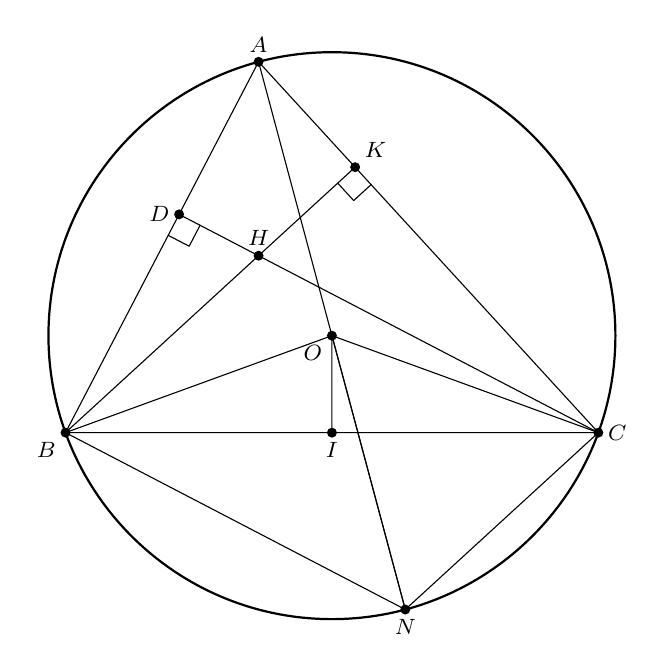
\begin{tikzpicture}[line join = round, line cap=round,>=stealth,font=\footnotesize,scale=1.2]
			\usetikzlibrary{calc,angles,quotes}
			% Def
			\def\r{3}
			
			% Coordinates
			\coordinate (O) at (0,0);
			\coordinate (A) at (105:\r);
			\coordinate (B) at (-160:\r); % or (200:\r)
			\coordinate (C) at (-20:\r);  % or (340:\r)
			
			% N such that O is midpoint of AN
			% N is A reflected through O, so N = -A (vector)
			% or N has angle of A + 180 deg
			\coordinate (N) at (105+180:\r); % or (-75:\r) or (285:\r)
			
			% I is midpoint of BC
			\coordinate (I) at ($ (B)!0.5!(C) $);
			
			% D is projection of C onto AB
			\coordinate (D) at ($ (A)!(C)!(B) $);
			
			% K is projection of B onto AC
			\coordinate (K) at ($ (A)!(B)!(C) $);
			
			% H is intersection of CD and BK (orthocenter of triangle ABC)
			% If O is circumcenter (which it is), H = A+B+C (vector sum from O)
			\coordinate (H) at ($ (A) + (B) + (C) $);
			
			% Draw
			% Draw circle (O,r)
			\draw[thick] (O) circle (\r);
			
			% Draw paths A-B-N-C-A-N-O-B-C-D-H-K-B
			\draw (A) -- (B) -- (N) -- (C) -- (A); % Quadrilateral ABNC and diagonal AC (actually CA)
			\draw (A) -- (N); 
			\draw (N) -- (O) -- (B);
			\draw (B) -- (C)--(O)--(I); 
			\draw (C) -- (D) -- (H) -- (K) -- (B);
			
			% Fill points
			\fill (O) circle (1.5pt);
			\fill (A) circle (1.5pt);
			\fill (B) circle (1.5pt);
			\fill (C) circle (1.5pt);
			\fill (N) circle (1.5pt);
			\fill (I) circle (1.5pt);
			\fill (D) circle (1.5pt);
			\fill (K) circle (1.5pt);
			\fill (H) circle (1.5pt);
			
			% Node points (old style)
			\node[below left] at (O) {$O$};
			\node[above] at (A) {$A$};
			\node[below left] at (B) {$B$};
			\node[right] at (C) {$C$}; 
			\node[below] at (N) {$N$}; 
			\node[below] at (I) {$I$}; % Adjusted for I on negative y-axis
			\node[left] at (D) {$D$};
			\node[above right] at (K) {$K$}; 
			\node[above] at (H) {$H$}; % Adjusted for H in Q2
			
			% Ky hieu goc vuong (old style)
			% CD is altitude to AB, so angle CDB or CDA is 90. C-D-B
			\pic[draw, angle radius=3mm]{right angle = B--D--C};
			% BK is altitude to AC, so angle CKB or AKB is 90. C-K-B
			\pic[draw, angle radius=3mm]{right angle = C--K--B};
			
		\end{tikzpicture}
		
	\end{center}
	}
\end{ex}

\begin{ex}
	\begin{enumerate}
		\item[a)] Một công ty Container cần thiết kế các thùng đựng hàng hình hộp chữ nhật, không nắp, có đáy là hình vuông, thể tích là 108m$^3$. Để tốn ít nguyên vật liệu nhất thì ta cần thiết kế các cạnh đáy của hình hộp bằng bao nhiêu?
		\item[b)] Cho a, b là các số thực dương thoả mãn $a + b = ab$. Tìm giá trị nhỏ nhất của biểu thức $P = \frac{1}{a^2+2a} + \frac{1}{b^2+2b} + \sqrt{(a^2+1)(b^2+1)}$.
	\end{enumerate}
\end{ex}


\setcounterref{ex}{0}